% !TEX root = main.tex
\chapter[head={The CKM angle $\gamma$},tocentry={The CKM angle $\symbfsf{\gamma}$}]{The CKM angle $\symbfsf{\gamma}$}
\label{ch:CKMAngleGamma}

As mentioned before overconstraining the triangle relations following from the unitarity of the matrix is a nice experimental self consistency check of the \ac{SM}.
The CKM angle $\gamma$ is one of five observables parametrising the CKM triangle described in \cref{eq:CKMtriangle}.
The current experimental constraints on this triangle are shown in \cref{fig:ckmtriangle}.
One can see that $\gamma$ is currently the least well known parameter.
Hence, a more accurate determination of $\gamma$ is one of the main tasks of current research in the field of flavour physics.
This chapter is organised as follows: Firstly it is described how $\gamma$ in general can be accessed in section \cref{sec:accessGamma}, especially the determination using tree-level decays (\cref{sec:gamamInTrees}) and loop-processes (\cref{sec:gamamInLoops}) is emphasized, followed by the explanation how the decay mode \BdToDpi can be used to derive constraints on $\gamma$ in \cref{sec:GammaInBd2Dpi}.

\begin{figure}[tbp]
	\centering
	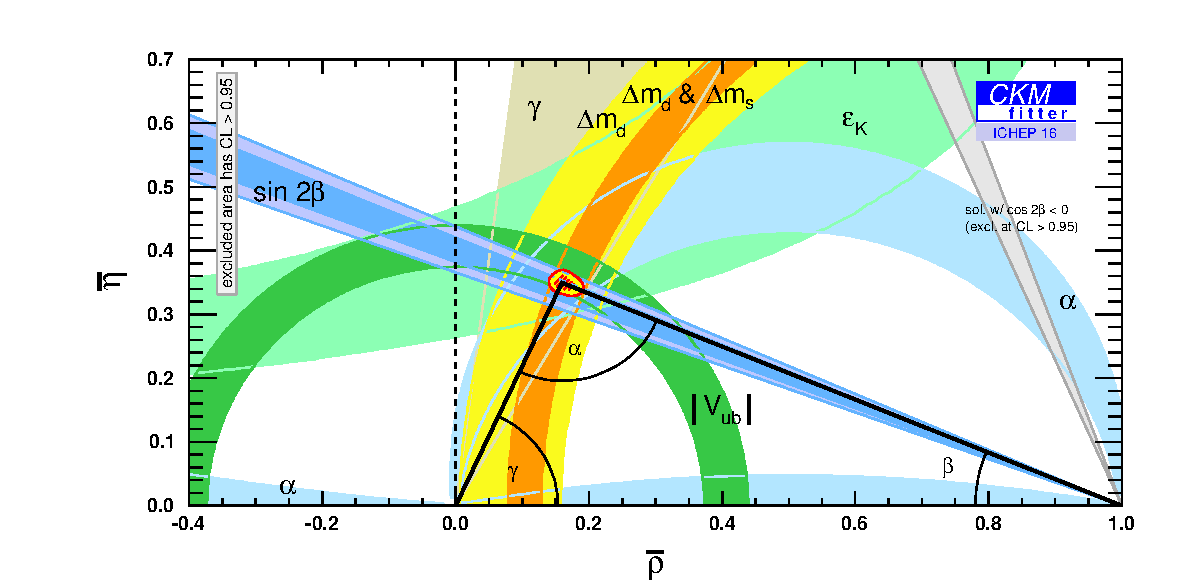
\includegraphics[width=0.8\textwidth]{04gamma/figs/CKMTriangle.pdf}
	\caption{CKM triangle in the complex plane.
	The coloured bands show the experimental constraints.
	The red hashed and the yellow area around the apex represent the currrent uncertainties at \SI{68}{\percent} and \SI{95}{\percent} confidence level, respectively~\cite{CKMfitter2015}.}
	\label{fig:ckmtriangle}
\end{figure}

\section[head={Accessing the angle $\gamma$},tocentry={Accessing the angle $\gamma$}]{Accessing the angle $\symbfsf{\gamma}$}
\label{sec:accessGamma}


As can be seen from the from in \cref{eq:CKMangles} the angle $\gamma$ is the only angle which is independent of CKM elements involving the top quark.
This makes it the only angle, which can be determined theoretically clean from tree-level decays.
On the other hand the experimental challenges are huge as transitions sensitive to $\gamma$ need to be proportional to \Vub, \ie such transitions are highly suppressed by order $\mathcal(O)\left(\lambda^3\right)$.
So either the precision of single measurements is limited due to small interference effects and branching fractions or in addition to the tree-level transition also penguin contributions of similar size contribute.
These gluonic penguins usually carry a weak phase different from the one in the tree-level diagram.

This latter possibility is briefly discussed using the example of the $\Bs\to\rho\KS$ decay.
Similar to the case of the golden mode \BdToJPsiKS, $\rho\KS$ is a \CP eigenstate and only the parameter \Lf needs to be calculated.
Using the amplitudes
\begin{equation}
\begin{aligned}
\Af&=\left<\rho\KS\left|T\right|\Bs\right>=-\frac{1}{2q_{\kaon}}\left<\rho\Kzb\left|T\right|\Bs\right>=-\frac{1}{2q_{\kaon}}\Vubst\Vud\\
\Abarf&=\left<\rho\KS\left|T\right|\Bsb\right>=\frac{1}{2p_{\kaon}}\left<\rho\Kz\left|T\right|\Bsb\right>=\frac{1}{2p_{\kaon}}\Vub\Vudst
\end{aligned}
\end{equation}
where $q_{\kaon}$ and $p_{\kaon}$ are the same mixing parameters for the neutral kaon system as shwon in \cref{eq:qoverp} for the \Bz-meson system.
With $\nicefrac{q_{\kaon}}{p_{\kaon}}=\nicefrac{\Vcsst\Vcd}{\Vcs\Vcdst}$ the parameter \Lf can be expressed in terms of the CKM matrix elements
\begin{equation}
\Lf=-\frac{q_{\kaon}}{p_{\kaon}}\frac{q}{p}\frac{\left<\rho\Kz\left|T\right|\Bsb\right>}{\left<\rho\Kzb\left|T\right|\Bs\right>}
=-\frac{\Vcsst\Vcd}{\Vcs\Vcdst}\frac{\Vtbst\Vts}{\Vtb\Vtsst}\frac{\Vub\Vudst}{\Vubst\Vud}.
\end{equation}
Using the Wolfenstein paramtrisation as shown in \cref{eq:CKMmatrix} this simplifies \Lf being a pure phase
\begin{equation}
\Lf=e^{-2i\gamma}.
\end{equation}
For $\Bs\to\rho\KS$ the finalstate $\rho$ has a \uquark\uquarkbar and a \dquark\dquarkbar component.
This means that alongside the spectator \squark-quark not only the tree-level transition $\bquark\to\uquark\uquarkbar\dquarkbar$ but also the gluonic-penguin transition $\bquark\to\dquark\dquarkbar\dquarkbar$ is possible (see \cref{fig:Bs2RhoKS}).
\begin{figure}[tbp]
	\centering
	\includestandalone{04gamma/figs/BsToRhoKS_Tree}
	\includestandalone{04gamma/figs/BsToRhoKS_Penguin}
	\caption{Tree-level diagram of $\Bs\to\rho\KS$ (left) and the dominantly contributing gluonic penguin (right). \cite{Ellis:2016jkw}.}
	\label{fig:Bs2RhoKS}
\end{figure}
For both diagrams the CKM-factor is $\propto A\lambda^3$, but the weak phases are $\gamma$ and $\beta$ for the tree-level diagram and the penguin, respectively.
The effect of an additional contributing amplitude with a weak phase differing from the one of the tree-level process can be quantified.
Considering two weak phases contributing to the transitions \Af ($\Bs\to\rho\KS$) and \Abarf ($\Bsb\to\rho\KS$):
\begin{equation}
\begin{aligned}
\Af&=A_1e^{i\left(\Phi_{A_1}+\delta_1\right)}+A_2e^{i\left(\Phi_{A_2}+\delta_2\right)}\\
\Abarf&=\eta_f\left[A_1e^{i\left(-\Phi_{A_1}+\delta_1\right)}+A_2e^{i\left(-\Phi_{A_2}+\delta_2\right)}\right]
\end{aligned}
\end{equation}
As shown in \cref{eq:qoverPPurePhase} the quantity $\nicefrac{q}{p}$ is a pure phase and hence one can write $\nicefrac{q}{p}=-e^{2i\Phi_\text{M}}$, what leads to
\begin{equation}
\Lf=-\eta_f\,e^{2i\Phi_\text{M}}\frac{ A_1 e^{i\left(-\Phi_{A_1}+\delta_1\right)} + A_2 e^{i\left(-\Phi_{A_2}+\delta_2\right)}}{A_1e^{i\left(\Phi_{A_1}+\delta_1\right)}+A_2e^{i\left(\Phi_{A_2}+\delta_2\right)}} \label{eq:LfWithPenguin}
\end{equation}
with the \emph{weak} and \emph{strong} phases $\Phi_{A_i}$ and $\delta_i$, respectively.
The phases $\Phi_{A_1}$, $\Phi_{A_2}$ and $\Phi_\text{M}$ are not rephasing-invariant, but the relative phases $\Phi_1\equiv\Phi_{A_1}-\Phi_\text{M}$, $\Phi_2\equiv\Phi_{A_2}-\Phi_\text{M}$ and $\Delta=\delta_2-\delta_1$ can be measured.
For $\Bs\to\rho\KS$ one can \eg identify $A_1$ and $A_2$ with amplitude corresponding to the tree-level and gluonic-penguin diagram, respectively.
Accordingly the phase $\Phi_1$ and $\Phi_2$ would represent the CKM angles $\gamma$ and $\beta$.
Already the form of $\Lf$ in \cref{eq:LfWithPenguin} shows that the penguin contribution in $\Bs\to\rho\KS$ makes it impossible to measure $\gamma$
However this case might be extrem in the sense that both amplitudes are of the same magnitude.
But even with the approximation that $r=\nicefrac{A_2}{A_1}$ is small one finds
\begin{align}
\Lf&=-\eta_fe^{-2i\Phi_1}\frac{1+re^{i\left(\Delta-\Phi_2+\Phi_1\right)}}{1+re^{i\left(\Delta+\Phi_2-\Phi_1\right)}}\nonumber\\
&\approx-\eta_fe^{-2i\Phi_1}\left[1+2r\sin\Delta\sin\left(\Phi_2-\Phi_1\right)-2ir\cos\Delta\sin\left(\Phi_2-\Phi_1\right)\right].
\end{align}
Obviously in case a guonic-penguin contributes with a different weak phase from that of the tree-level diagram - \ie $r\neq0$ and $\Phi_1\neq\Phi_2$ - it is not possible to measure a single weak phase.
Now one finds, that in case a second penguin with a different weak phase from that of the tree-level diagram contributes the parameter and $r\neq0$, \Lf does not allow to measure a single weak phase.
Even in the case of vanishing final state interactions, \ie $\Delta=0$, \Lf can just be written as
\begin{equation}
\Lf=-\eta_fe^{-2i\left(\Phi_1-\delta_{\Phi_1}\right)}
\end{equation}
where $\delta_{\Phi_1}$ is defined by
\begin{equation}
\tan\left(\delta_{\Phi_1}\right)=\frac{r\sin\left(\Phi_1-\Phi_2\right)}{1+r\cos\left(\Phi_1-\Phi_2\right)}.
\end{equation}
Additionally it is important to note that hadronic matrix elements cannot be calculated reliably.
This means that in case they do not cancel out as they do if only one amplitude contributes to a specific decay, the resulting \CP asymmetries cannot be interpreted without large uncertainties which need to be propagated into the determination of the sides and angles of the unitarity triangle.

Therefore the current strategy to decrease the uncertainty on $\gamma$ is to measure it in many different decay modes and combine the results afterwards.
These decay modes can be divided into the two mentioned classes: The first class are tree-level processes where either decays of charged \B mesons or neutral \B mesons are exploited.
The second class are processes involving penguin contributions, \eg similar to the contribution to $\Bs\to\rho\KS$ described above.

\subsection[head={Determination of $\gamma$ in tree-level decays},tocentry={Determination of $\gamma$ in tree-level decays}]{Determination of $\symbfsf{\gamma}$ in tree-level decays}
\label{sec:gamamInTrees}

% In the \ac{SM} two types of \CP violation, namely direct and interference \CP violation, are expected to a non-negligible amount.
As $\gamma$ is propotional to the phase of the matrix element \Vub a natural way to measure it is to exploit interference effects between the Cabibbo-favoured $\bquark\to\cquark$ transitions and the Cabibbo-suppressed $\bquark\to\uquark$ transitions in decay channels such as $\Bu\to\D\Kp$ and \BsToDsK.
In the first case exploring different \D decay chaines requires slightly different experimental methods, whereas in the latter case a time-dependent analysis is needed.

The basic principle when exploiting decays of charged \B mesons is always the same.
The initial \Bpm meson decays into \Dz\Kpm or \Dzb\Kpm and subsequently the \D meson is reconstructed in a final state common to both \Dz and \Dzb.
Therefore the amplitudes for the decay of the \B meson can be defined as
\begin{equation}
\begin{aligned}
A\left(\Bp\to\Dz\Kp\right)&=\Vubst\Vcs=Ae^{i\left(\delta+\gamma\right)}\\
A\left(\Bp\to\Dzb\Kp\right)&=\Vcbst\Vus=\overline{\kern -1.0pt A\kern -1.0pt}\,e^{i\left(\overline{\delta}\right)}
\end{aligned}
\end{equation}
where the \emph{weak} phase was directly idenitified as $\gamma$, $\delta$ and $\overline{\delta}$ are the \emph{strong} phases and $A$ and $\overline{\kern -1.0pt A\kern -1.0pt}$ are the moduli of the amplitudes.
For the \D-meson decay the ampltiudes can be defined accordingly as
\begin{equation}
\begin{aligned}
A\left(\Dz\to\f\right)&=A_De^{i\left(\delta_D\right)}\\
A\left(\Dzb\to\f\right)&=\overline{\kern -1.0pt A\kern -1.0pt}_D\,e^{i\left(\overline{\delta}_D\right)}.
\end{aligned}
\end{equation}
Hence, the transition of $\Bp\to\f$ has two contributing amplitudes, which produce an interference term in the total decay rate
\begin{equation}
\left|A\left(\Bp\to\f\,\Kp\right)\right|^2=\overline{\kern -1.0pt A\kern -1.0pt}{}^2A_D^2+A^2\overline{\kern -1.0pt A\kern -1.0pt}{}_D^2+2\,\overline{\kern -1.0pt A\kern -1.0pt}{}^2A_D^2A^2\overline{\kern -1.0pt A\kern -1.0pt}{}_D^2\cos\left(\gamma+\Delta+\Delta_D\right)
\end{equation}
where the short notation $\Delta=\overline{\delta}-\delta$ and $\Delta_D=\delta_D-\overline{\delta}_D$ were used.

The first method exploiting decays of charged \B mesons is the so-called GLW method \cite{GLW_1, GLW_2}.
It should be noted that the same procedure can be applied to decays as $\Bpm\to\D\pipm$.
% In \cref{sec:gammainChargedModes} methods for decays which suffer direct \CP violation as the $\Bu\to\Dz\Kp$ or the $\Bu\to\Dz\Kp\pip\pim$ as the GLW and the GGSZ method will be discussed.

\subsection[head={Determination of $\gamma$ in loop processes},tocentry={Determination of $\gamma$ in loop processes}]{Determination of $\symbfsf{\gamma}$ in loop processes}
\label{sec:gamamInLoops}
Read the fleischer paper and understand the experimental status

\subsection[head={Comparison of tree-level and loop determinations of $\gamma$},tocentry={Comparison of tree-level and loop determinations of $\gamma$}]{Comparison of tree-level and loop determinations of $\symbfsf{\gamma}$}

\section[head={Measuring $\gamma$ in $\Bz\to\Dm\pip$},tocentry={Measuring $\gamma$ in $\Bz\to\Dm\pip$}]{Measuring $\symbfsf{\gamma}$ in $\symbfsf{\Bz\to\Dm\pip}$}
\label{sec:GammaInBd2Dpi}
